%%%%%%This is a very basic LaTex Template created for your assignments%%%%%
\documentclass[12pt]{article}
\usepackage{geometry}
\usepackage{graphicx}
\usepackage{epsfig}
\usepackage{amsfonts, amsmath, amssymb, marvosym,appendix,color,hyperref}
\geometry{top=1in, bottom=1in, left=1in, right=1in}
\usepackage{verbatim}
\usepackage{setspace}
\onehalfspacing
\pagestyle{plain}
\usepackage{natbib}
\bibpunct{(}{)}{,}{a}{,}{;} 
\bibliographystyle{agsm}
\usepackage{subcaption}



\hypersetup{
    colorlinks=false, %true will add colored links
    linktoc=all,     %all will add links to all sections and subsections.
    linkcolor=red,  %the colour you want to use for your link so that it stands out
}




\title{How Weather Can Affect the Game} % Insert your title here

\author{Michael Bubniak, Tianheng Chen, Akira Taniguchi} %Name of the author

\date{\today} %You can either specify a date or leave it empty. If left empty, the date of compilation will be used.



\begin{document}
\maketitle

\newpage

\tableofcontents


\newpage

\section*{Abstract}
This article will discuss the affects that different elements of weather has on a football game. It is a common belief that it is harder to play football in certain weather conditions, and ideal in other conditions. The "ideal" condition is presumed to be no wind, no precipitation and the average temperature of a given teams hometown. The data is drawn from every NFL game (that has retrievable data) from the 2015 season to the 2018 season. The weather is broken up into the wind, humidity, game day temperature, temperature difference from the teams hometown and a binary precipitation measure. A given teams performance is gauged on how many offensive yards are gained in rushing, passing and total. Defensive performance is measured in a similar manner, but instead a better performance is having lesser yards allowed for the opposing team. There is also a binary dome measurement, as playing in a dome is in a controlled environment and the field is not subject to the weather outside. 


\section{Introduction}\label{intro}

\quad With the technology explosion that has been happening in recent times, the amount of information that somebody can keep track of has exponentially grown. Over the past several decades, professional sports have taken advantage of this ability and kept track of more data than ever before. In theory, the more data that an athletic team has, the more they can manipulate their game plan to what the data dictates, which allows for better performance for the team and the individuals on the team. Some recent examples of this include the “shift” in baseball fielding, quarterback rating for passing or rushing for football, and zone defense changes in basketball. This allows for teams to have a greater knowledge of the opposing team and perform accordingly to each given scenario.

A much more universal dictator of the game is the weather conditions. Regardless of what the sport is (unless it’s indoors), the players are victims of the weather for gameday. Muscle flexibility is ideal in specific weather conditions, it is much easier to throw a ball or gather grip on the field when running in dry weather, how points are scored vary with the weather, and many other variables. In the NFL, the weather is incredibly sporadic, as the season takes place from August to February, which have polar opposite weather conditions, and games take place all over the country; a game in Jacksonville is much different than a game in Green Bay played at the same time. If a home team knows that their opponents are not acclimated to their weather and it causes the team to perform differently, the home team will use this to their advantage. Knowing how the weather can affect the opposing individuals or the opposing team as a whole can create a large advantage for the team in the know, as they now have the ability to shift their strategies to combat what the other team brings to the table.

To answer how the weather can affect a player or team performance, many variables can be looked at. With the availability of almost all statistics on every football game along with what the weather conditions were, correlations and trends can be found. The overall performance of a team can be characterized by how “well” its offense performs along with how its defense performs. Naturally, offense performance is characterized by how many points are scored along with, how many rushing yards and how many passing yards, all of these subject to the weather. Defense is essentially measured in the opposite manner, in that less passing and rushing yards are better while allowing less points. There is also the factor of playing in a dome, as the weather conditions don’t affect the field as extreme versus an open field. With these two data sets, weather and performance, an analysis can be made to compare how each component of the weather affects each component of the performance. It then can be looked at to see how performance is affected as a whole. With these results, it then can be shown how much the weather affects the game and what useful information can come of it.

Weather itself also has a variety of variables that can affect the gameplay. The variable that has the largest variance is the temperature. A player on Jacksonville will most likely be acclimated to extreme heat in the early months of the season, but also not used to the extreme cold that Buffalo can provide in the later months of the year. For the Florida native, playing in January in the north might cause them to not be as agile or quick due to their muscle flexibility not being able to handle the change of temperature. The Buffalo native however trains in the cold and is bred by the cold, so they will have a higher tolerance for the frost that a harsh winter can bring. Conversely, Buffalo players are used to snow and negative temperatures, or at least able to handle them better than a person that is accustomed to sunny Florida, but extreme heat in the earlier part of the season might affect the northerner harder. Extreme heat causes exhaustion faster and can also cause over-flexibility in muscles (rare but possible), which a Jacksonville player has dealt with on a regular basis and will have a higher tolerance than the player from Buffalo. Humidity has also has a similar affect on players, as one can become accustomed to a specific air quality. Deviating from one's ideal temperature or playing in an extreme humidity can cause performance hindrances and affect how the game is played.

There is also the "storm" elements of the weather, wind and precipitation. In an extreme case, where wind is strong enough to drastically alter the path of a football in the air, coaches would be inclined to call plays that dictate not throwing the ball, as it would be harder to throw with accuracy. Similarly, throwing in the rain or snow is also not ideal, as the ball loses much of it's grip and extreme precipitation can slow down the ball in the air. These factors will lead to more rushing as opposed to passing the ball. Rushing itself is also not ideal in harsh weather, as the field does not have a lot of grip. This creates a slower paced game as most activity has to be slowed down to perform properly. But, all of this variation can be blocked with a dome field, which a handful of teams have, such as Detroit and Minnesota. A dome has a controlled temperature and humidity so players are always comfortable and don't have to worry about the possibility of storms and the harsh conditions that they bring.

A similar study, done in the article \textit{Effect of Cold Weather on NFL Game} by Brian Nemhauser, looks at how the temperature affects the teams performance in a football game for the Seattle Seahawks. Nemhauser finds that the colder a game is, the less points are scored, the more turnovers happen and the average yards gained drops. With this information, it can be gathered that it is harder to play in colder weather, as it is known that muscle activity is not ideal in colder weather, which is backed up by these findings. Similar results were found by Brian Burke in his article \textit{Weather Effects on Passing}, in that colder weather and snowier conditions create difficulty in passing mechanics, which lead to less passing in harsher weather.

\section{Methodology}\label{method}
\quad Statistically, how "good" an NFL team performs as a whole can be looked at by their final yardage, in both offense and defense. The better one's offense performs, the more yardage they will have and inversely for the defense, in that they ideally want to give up less yards to the opposing team. As with most statistics, this isn't completely true. A team can theoretically drive up the field every possession, but for unpredictable reasons, not score at all (something like a fumble or interception at the endzone) creating a statistically amazing performance but a realistic not that great performance. Similarly, the defense could only let up 100 yards and 1 field goal, an amazing performance, but the offense doesn't score so it's a loss. But, these are far and few between, so given enough data, by using every single game from 2015 onwards, they will not affect the data enough to cause concern. For this model, it will be assumed that a teams performance will be based on their offense's ability to produce yards and the defense to prevent yards.

\quad For the weather, it can be broken up into wind speed, temperature difference, and humidity with binary results for playing in a dome and rain. Wind speed and humidity are self-explanatory, as each data point is it's face-value on what is going on. The dome and precipitation variables are treated as dummy variables for the model, as there is no other measure to a dome besides it's existence and the amount of rain on given days is difficult to pinpoint. Temperature is slightly more complicated. Using just the degree amount on a given day only explains what a theoretical performance should be to the NFL as a whole, but doesn't explain what a team is adapted to. For a team the is used to playing in the heat, it might show a positive relationship with the temperature, against a team that has a tolerance for the cold which would show an inverse relationship with the temperature. To accommodate this, the average temperature of each hometown is gathered from \textit{usclimatedata.com} and attached to it's respective team. The absolute value of the difference between the average temp and the gameday temp is then used as the temperature difference.

\quad The information for the result of each game exists on \textit{profootballreference.com}. This provides the sample with each section of defense and offense yardage for every game since 2015. Comparing this with the weather info for each day and city that a game takes place in, is provided by \textit{sportradar.com}, the data can take it's shape. Any information that wasn't given or anything that was given as an error was removed from the model, as it is assumed that data from that day was either not reported or reported incorrectly. Games that are in a dome are in a controlled environment, which according to \textit{sportradar.com} is at 68 degrees and 70\% humidity. So if a game takes place in a dome, that is the assumed conditions and the dome dummy is listed accordingly. Using the data gathered from these two sources, models can be derived and results can be gathered. 

\section{Results and Discussion}\label{result}

\subsection{Passing Versus the Weather}
In this section, the effects that the weather will have on the passing yards will be shown.

As shown in the figures, there is a slight increase with passing yardage versus temperature. This makes sense because, within a certain limit, the warmer the weather is, the better one performs. Playing in colder temperatures tends to be harder to stay flexible and slows muscle twitch time, dampening the results that will come out of the players. Humidity showed to not have that much of an effect on how many yards should be gained. With the remaining variables, difference, dome, precipitation and wind, there was a negative correlation. There is logic to these results as it would make sense for higher winds and more rain/snow to make it harder to throw a ball. There is also the added effect of having a greater difference in temperature to lessen the amount of yards that are being produced.

With the residual plots, all of them appear to have a linear relationship. All of the linear relationships also appear to be very strong in nature. This implies that the data generally has a linearly relationship with the variables. The values when independently comparing measurements that were significant (at a 5\% level) were Temperature(.3489), Difference(-.5123), Precipitation(-17.609), and Dome(24.969). When a full model was ran that combined all of the variables into one equation, the significant variables were Temperature(.35821), Humidity(.1931), Difference(-.55), and Precipitation(-21.47955).

\begin{figure}[h!]
	\centering
	\begin{subfigure}[b]{0.4\linewidth}
		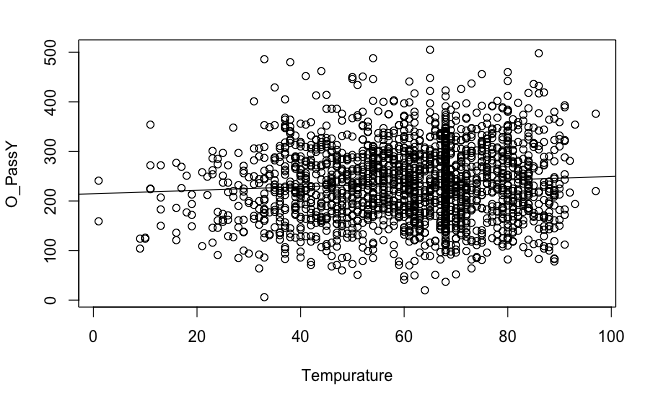
\includegraphics[width=\linewidth]{N_pass_temp.png}
	\end{subfigure}
	\begin{subfigure}[b]{0.4\linewidth}
		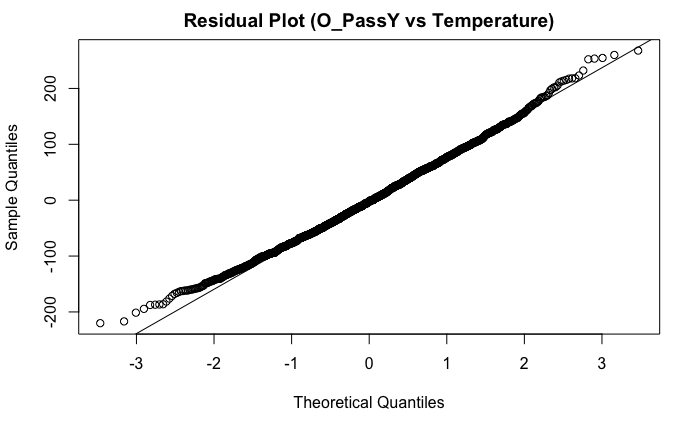
\includegraphics[width=\linewidth]{R_pass_temp.png}
	\end{subfigure}
\end{figure}

\begin{figure}[h!]
	\centering
	\begin{subfigure}[b]{0.4\linewidth}
		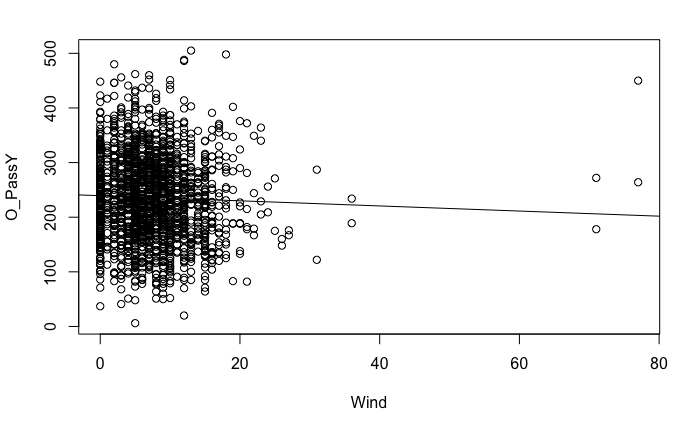
\includegraphics[width=\linewidth]{N_pass_wind.png}
	\end{subfigure}
	\begin{subfigure}[b]{0.4\linewidth}
		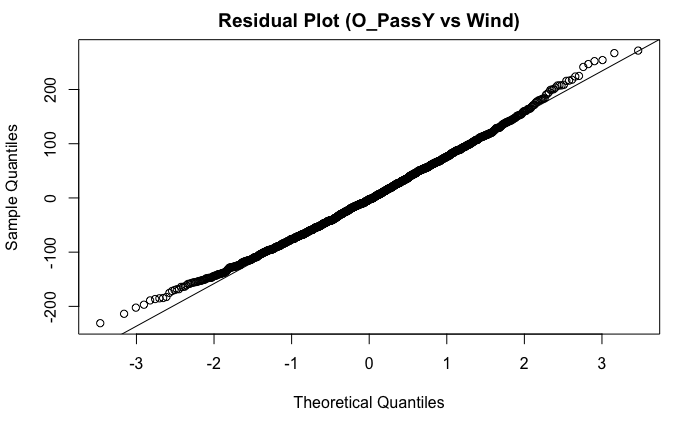
\includegraphics[width=\linewidth]{R_pass_wind.png}
	\end{subfigure}
\end{figure}

\begin{figure}[h!]
	\centering
	\begin{subfigure}[b]{0.4\linewidth}
		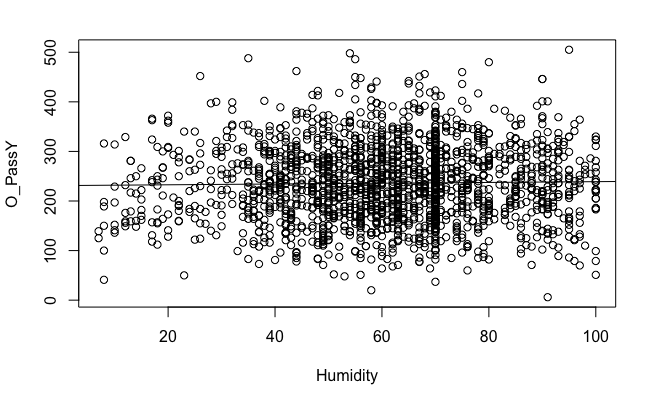
\includegraphics[width=\linewidth]{N_pass_hum.png}
	\end{subfigure}
	\begin{subfigure}[b]{0.4\linewidth}
		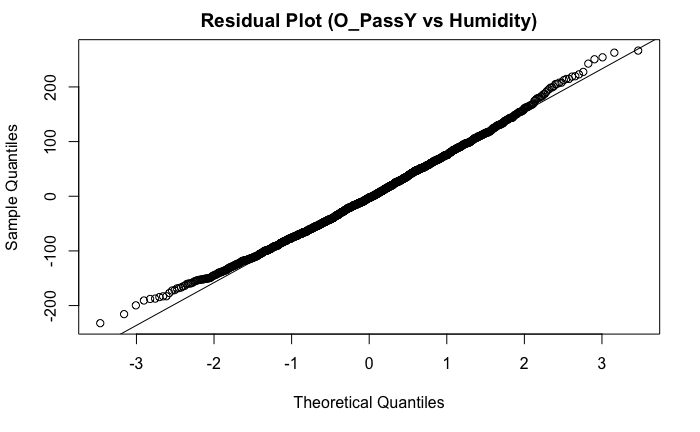
\includegraphics[width=\linewidth]{R_pass_hum.png}
	\end{subfigure}
\end{figure}

\begin{figure}[h!]
	\centering
	\begin{subfigure}[b]{0.4\linewidth}
		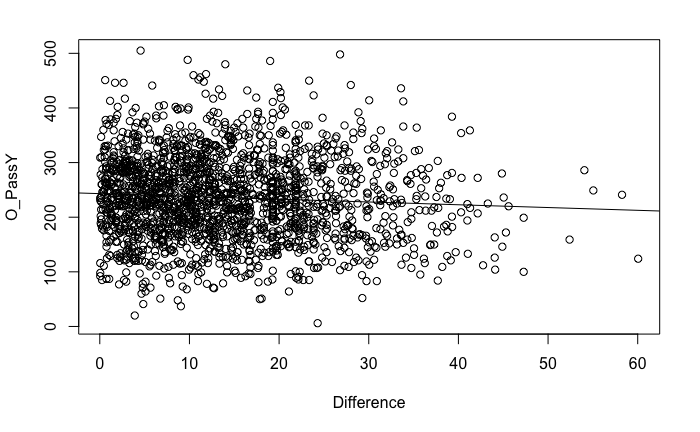
\includegraphics[width=\linewidth]{N_pass_diff.png}
	\end{subfigure}
	\begin{subfigure}[b]{0.4\linewidth}
		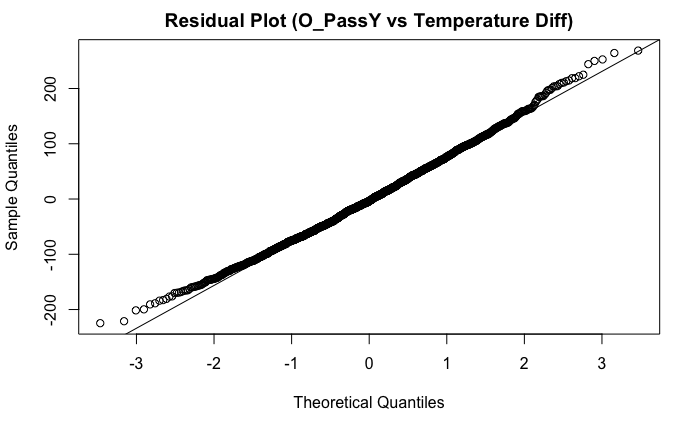
\includegraphics[width=\linewidth]{R_pass_diff.png}
	\end{subfigure}
\end{figure}

\begin{figure}[h!]
	\centering
	\begin{subfigure}[b]{0.4\linewidth}
		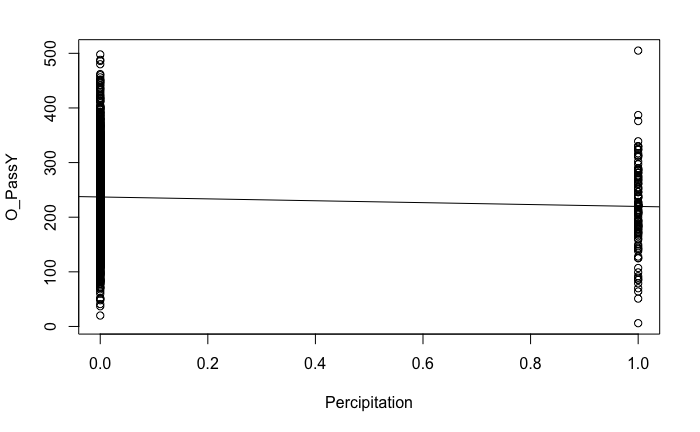
\includegraphics[width=\linewidth]{N_pass_perc.png}
	\end{subfigure}
	\begin{subfigure}[b]{0.4\linewidth}
		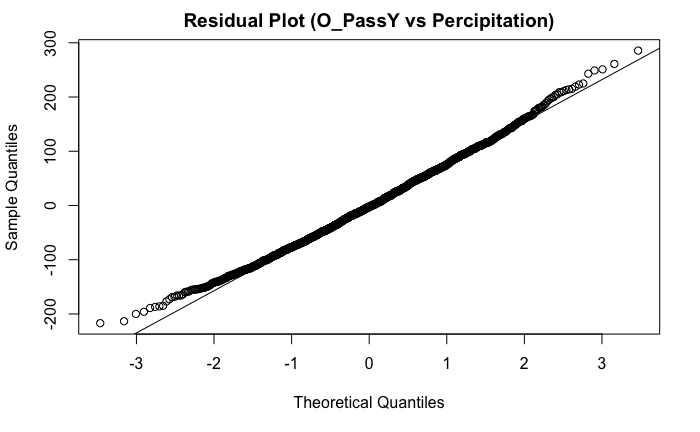
\includegraphics[width=\linewidth]{R_pass_perc.png}
	\end{subfigure}
\end{figure}

\begin{figure}[h!]
	\centering
	\begin{subfigure}[b]{0.4\linewidth}
		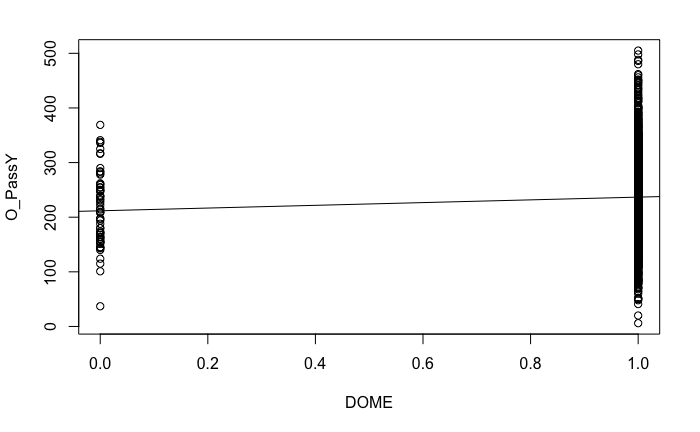
\includegraphics[width=\linewidth]{N_pass_dome.png}
	\end{subfigure}
	\begin{subfigure}[b]{0.4\linewidth}
		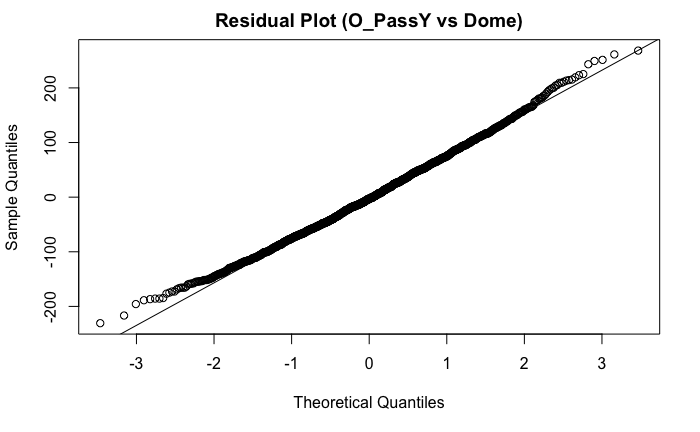
\includegraphics[width=\linewidth]{R_pass_dome.png}
	\end{subfigure}
\end{figure}



\subsection{Rushing Versus the Weather}
In this section, the effects that the weather will have on the rushing yards will be shown.

\quad Compared to the passing results, the weather has some different effects on the rushing. Humidity and difference appear to have no difference to the effect on rushing output. Wind and precipitation have a positive effect on the rushing performance. This isn't necessarily an direct relationship however. A shown before, these two have a negative effect on passing yards. This displays that it is much harder to throw a ball in storm conditions than in calmer weather. The only other way to safely produce yards without giving up interceptions or fumbles is to run the ball. In essence, it isn't easier to run the ball in a hurricane, but it is much easier than throwing the ball.

With the residual plots, all of them appear to have a linear relationship. All of the linear relationships also appear to be very strong in nature, but not as strong as the passing residuals. This implies that the data has a linearly relationship, with their respective variables, but not as strongly correlated as it's passing counterpart. The variables that were at a significant (at a 5\% level) were Temperature(-.20657) and Precipitation(8.311). With the full model, the significant variable was only Temperature(-.19986)

\begin{figure}[h!]
	\centering
	\begin{subfigure}[b]{0.4\linewidth}
		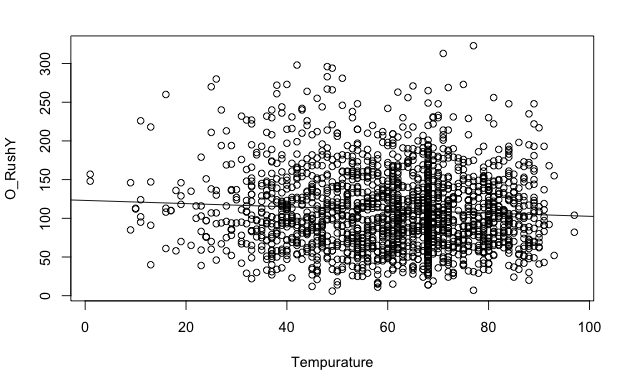
\includegraphics[width=\linewidth]{N_rush_temp.png}
	\end{subfigure}
	\begin{subfigure}[b]{0.4\linewidth}
		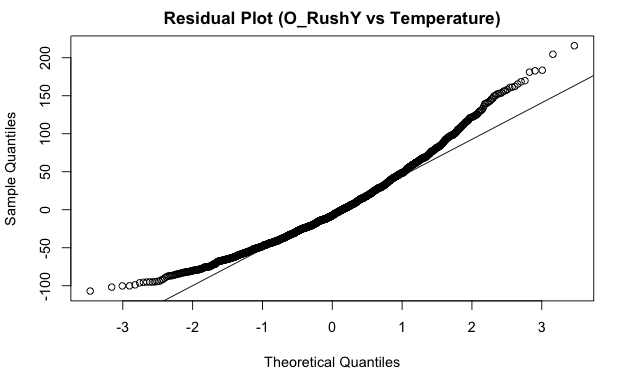
\includegraphics[width=\linewidth]{R_rush_temp.png}
	\end{subfigure}
\end{figure}

\begin{figure}[h!]
	\centering
	\begin{subfigure}[b]{0.4\linewidth}
		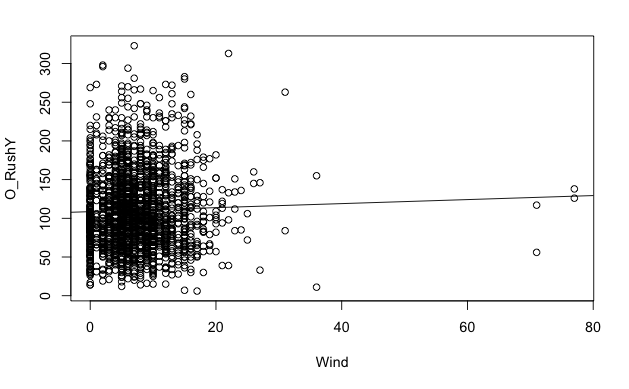
\includegraphics[width=\linewidth]{N_rush_wind.png}
	\end{subfigure}
	\begin{subfigure}[b]{0.4\linewidth}
		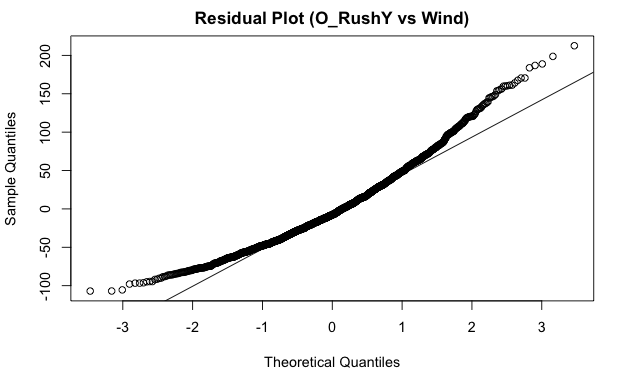
\includegraphics[width=\linewidth]{R_rush_wind.png}
	\end{subfigure}
\end{figure}

\begin{figure}[h!]
	\centering
	\begin{subfigure}[b]{0.4\linewidth}
		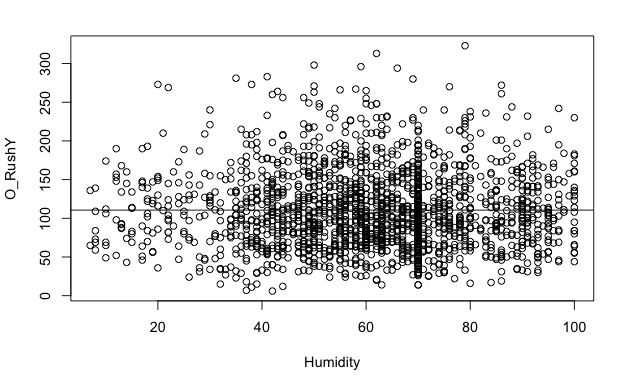
\includegraphics[width=\linewidth]{N_rush_hum.png}
	\end{subfigure}
	\begin{subfigure}[b]{0.4\linewidth}
		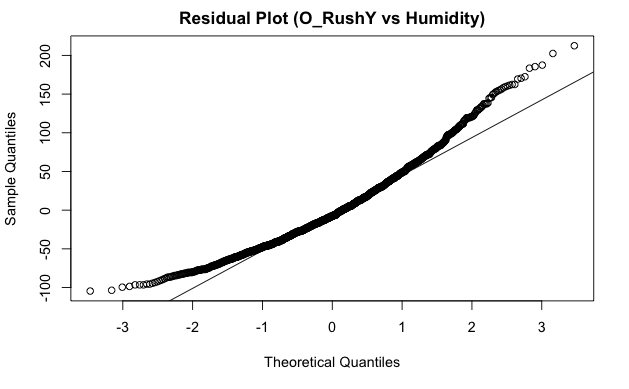
\includegraphics[width=\linewidth]{R_rush_hum.png}
	\end{subfigure}
\end{figure}

\begin{figure}[h!]
	\centering
	\begin{subfigure}[b]{0.4\linewidth}
		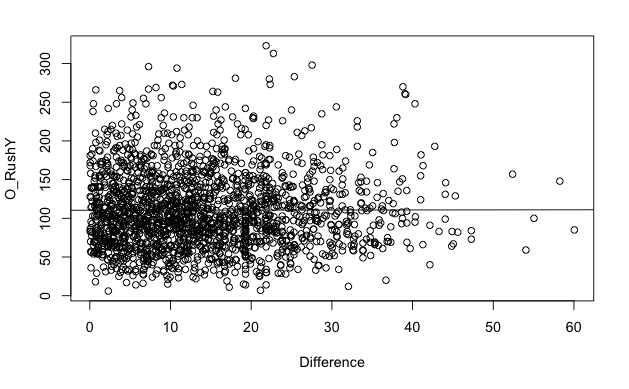
\includegraphics[width=\linewidth]{N_rush_diff.png}
	\end{subfigure}
	\begin{subfigure}[b]{0.4\linewidth}
		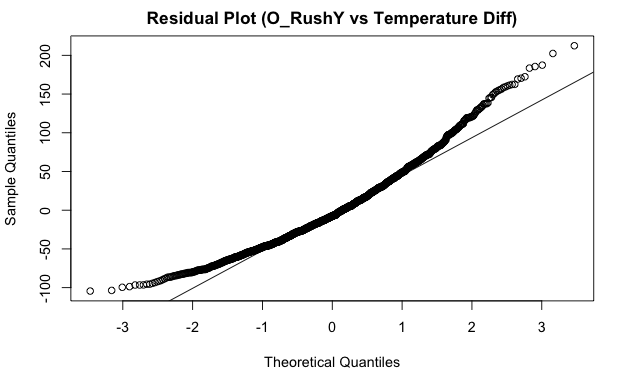
\includegraphics[width=\linewidth]{R_rush_diff.png}
	\end{subfigure}
\end{figure}

\begin{figure}[h!]
	\centering
	\begin{subfigure}[b]{0.4\linewidth}
		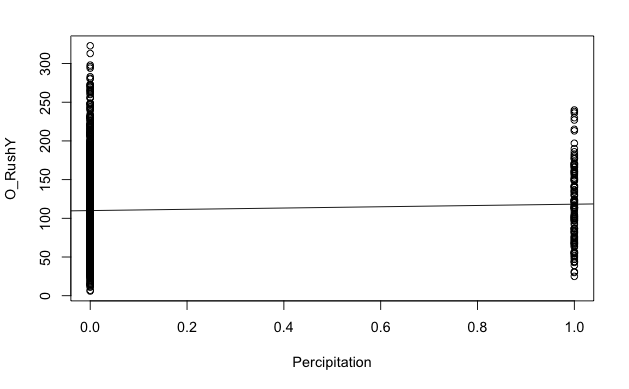
\includegraphics[width=\linewidth]{N_rush_perc.png}
	\end{subfigure}
	\begin{subfigure}[b]{0.4\linewidth}
		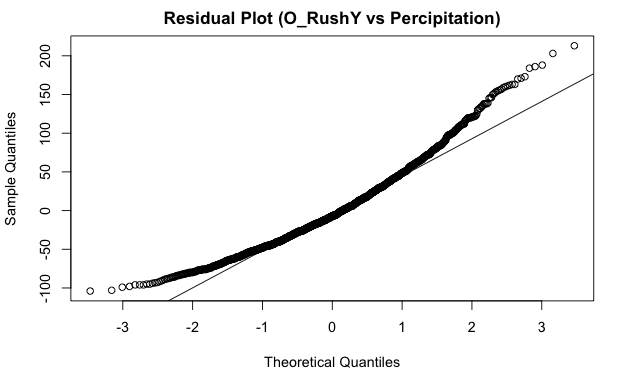
\includegraphics[width=\linewidth]{R_rush_perc.png}
	\end{subfigure}
\end{figure}

\begin{figure}[h!]
	\centering
	\begin{subfigure}[b]{0.4\linewidth}
		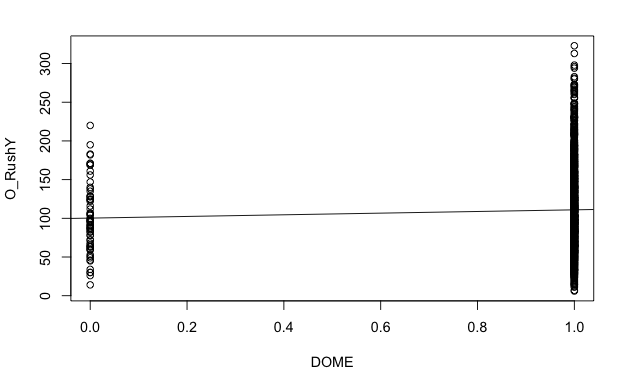
\includegraphics[width=\linewidth]{N_rush_dome.png}
	\end{subfigure}
	\begin{subfigure}[b]{0.4\linewidth}
		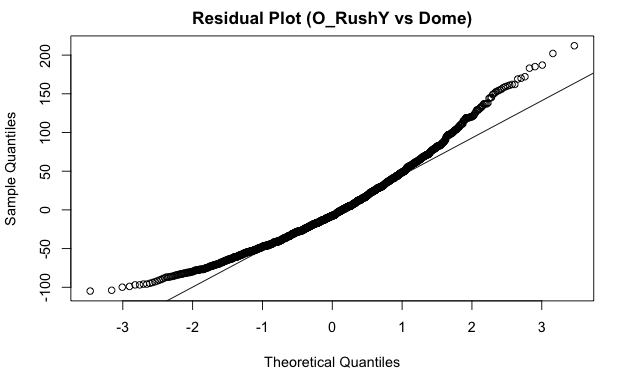
\includegraphics[width=\linewidth]{R_rush_dome.png}
	\end{subfigure}
\end{figure}



\subsection{Without the Dome}
\quad To see if having no dome games created a different result, the games that were played in a dome were removed from the model. This creates the measurements with the remaining data to be only games that are actually affected by the weather and leaves out any that have a "cushioned" environment. The games that were described as playing in a dome were 32, which in the data is 64 values, as each game is listed twice to account for each teams offense performance. With the full model without the dome, the significant variable were Temperature(.38295), Humidity(.22668), Difference(-.5632) and Precipitation(-23.30743) for passing. For rushing, the only variable that was significant was Temperature(-.19444).
\section{Conclusion}
\quad Models with a dome have a decrease in yardage and it is not intuitive as to why there is a negative correlation. It would be thought to have a positive impact on players to be in a controlled environment than to have a negative one. The assumed reason behind this is that modeling with the dome variable will have the majority effect on the teams that have dome's as there home field, like the Detroit Lions for example. These teams will have the most impact on the dome data, causing the dome to model what Detroit is doing instead of the NFL as a whole. In our case, it just happened that the dome having teams in this data performed poorly for the time frame that was given. With this non-expected result, a model without any game that had a dome, to analyze if there was a better correlation to the data with the other existing variables.

Defense was decided to be removed from the final display for repetitive reasoning. Due to every game being looked at from both perspectives, home and away teams, the defensive performance by one team in a game would be mirrored by the offensive performance from the other team in the same game. When executed by the code, this was confirmed to show the same results for all of the coefficients and displays in the graphs.

Wind, while not being significant in any scenario, was drastically improved with the progression of the models with respect to it's p-value. Between the two models for rushing, including the dome dropped the p-value by more than .3, which is a great improvement. For rushing yardage, with all of the combinations, the best r-squared value came out of using temperature, precipitation and humidity, with an adjusted r-squared of .005.

For all of the models, it was shown that temperature was significant. This implies that temperature is the most impacting variable. Not in the sense of the most yards were gained or lost, but that the temperature during gameday is the variable in the weather that can be most relied on to decipher the outcome of the game. With all of the models, there was also an issue with the R-squared values, as all of them were below 5\%. This gives the implication that most of the variation to the game is provided by other elements of the game. It is also implied with this that trying to predict the outcome of a game based exclusively on weather, is near impossible. If the model were to be ran again, more variables would have to be considered to get a more definitive prediction scheme. While it may not be exact, there are a couple inches to be gained in the game from using the weather as a basis.

\section{Bibliography}
Nemhauser, B. (2016, January 7). Effect of Cold Weather on NFL Games. Retrieved from http://www.hawkblogger.com/2016/01/effect-of-cold-weather-on-nfl-games.html.

Burke, B. (n.d.). Weather Effects on Passing. Retrieved from

 http://archive.advancedfootballanalytics.com/2012/01/weather-effects-on-passing.html.

Park, E. (n.d.). Weather and the NFL. Retrieved November 22, 2019, from

 https://web.stanford.edu/class/stats50/projects16/Houghton-BerryParkPierce-paper.pdf.

https://www.usclimatedata.com/climate/united-states/us

https://www.sportradar.com

https://www.profootballreference.com

\begin{appendices}
 \section{Python Code to Gather Data}
 \begin{verbatim}
 import pandas as pd
 urlhead = 'http://www.pro-football-reference.com/teams/'
 urltail = '.htm'
 newcolumns=['Week','Day','Date','NA1','NA2','W/L','NA4','REC','LOC','Opp'
 ,'Score_Team','Score_Opp','O_1stD','O_TotYd','O_PassY','O_RushY','O_TO',
 'D_1stD','D_TotYd','D_PassY','D_RushY','D_TO','Expected_O_Pts',
 'Expected_D_Pts','Expected_Sp_Pts']
 drop = ['Day','REC','NA1','NA2','NA4','Expected_O_Pts',
 'Expected_Sp_Pts','Expected_D_Pts','O_TO','D_TO','O_1stD','D_1stD']
 allteams = ["ram","den","sea","sfo","atl","sdg","kan","car","nyg","was",
 "nor","min","tam","nwe","buf","nyj","mia","rav","pit","cle","cin","htx",
 "clt","oti","jax","rai","dal","phi","gnb","chi","det","crd"]
 allyears = ["2009","2010","2011","2012","2013","2014","2015",
 "2016","2017","2018"]
 def createDF(url):
 dfs = pd.read_html(url)
 df = dfs[1]
 df.columns = [' '.join(col).strip() for col in df.columns.values]
 df.columns=newcolumns
 df['LOC'] = df['LOC'].fillna(value=0)
 df['LOC'] = df['LOC'].replace(0,'Home')
 df['LOC'] = df['LOC'].replace('@','Away')
 df=df.drop(drop,axis=1)
 bye_idx = df.index[df['Opp'].str.match('Bye',na=False)]
 df = df.drop(bye_idx,axis = 0)
 df = df.head(16)
 df.set_index('Week')
 return df
 def csvLoop():
 for x in range(len(allteams)):
 team = allteams[x]
 for y in range(len(allyears)):
 year = allyears[y]
 url = urlhead + team + '/' + year + urltail
 file = team + '_' + year + '.csv'
 createDF(url).to_csv(file,index=False)
 csvLoop()
 \end{verbatim}
  \section{Code From R}
   \begin{verbatim}
  ```{r}
  b<-ggplot(Master1,aes(Difference))
  b+geom_area(stat = "bin")
  ```
  ```{r}
  Master2=Master1[,5:19]
  qqplot(unlist(Master2[,9]),unlist(Master2[,5]))
  qqplot(unlist(Master2[,9]),unlist(Master2[,4]))
  qqplot(unlist(Master2[,10]),unlist(Master2[,5]))
  qqplot(unlist(Master2[,10]),unlist(Master2[,4]))
  qqplot(unlist(Master2[,11]),unlist(Master2[,5]))
  qqplot(unlist(Master2[,11]),unlist(Master2[,4]))
  qqplot(unlist(Master2[,4]),unlist(Master2[,5]))
  qqplot(DOME,O_RushY)
  ```
  ```{r}
  summary(x<-lm(O_PassY~Tempurature+Humidity+DOME+Wind+Difference+Percipitation
  ,Master1))
  summary(y<-lm(O_PassY~Tempurature+Humidity+I(DOME*Wind)+Difference+Percipitation
  ,Master1))
  summary(n<-lm(O_PassY~Tempurature+Humidity+Wind+Difference+Percipitation
  ,Master1))
  cor(Master2[,9:15])
  abline(0,0,col=2)
  vif(x)
  vif(n)
  ```
  \end{verbatim}

\end{appendices}



\end{document}